\begin{frame}{Альтернированная цепочка}
\begin{columns}

    \column{0.3\textwidth}
    \begin{figure}
    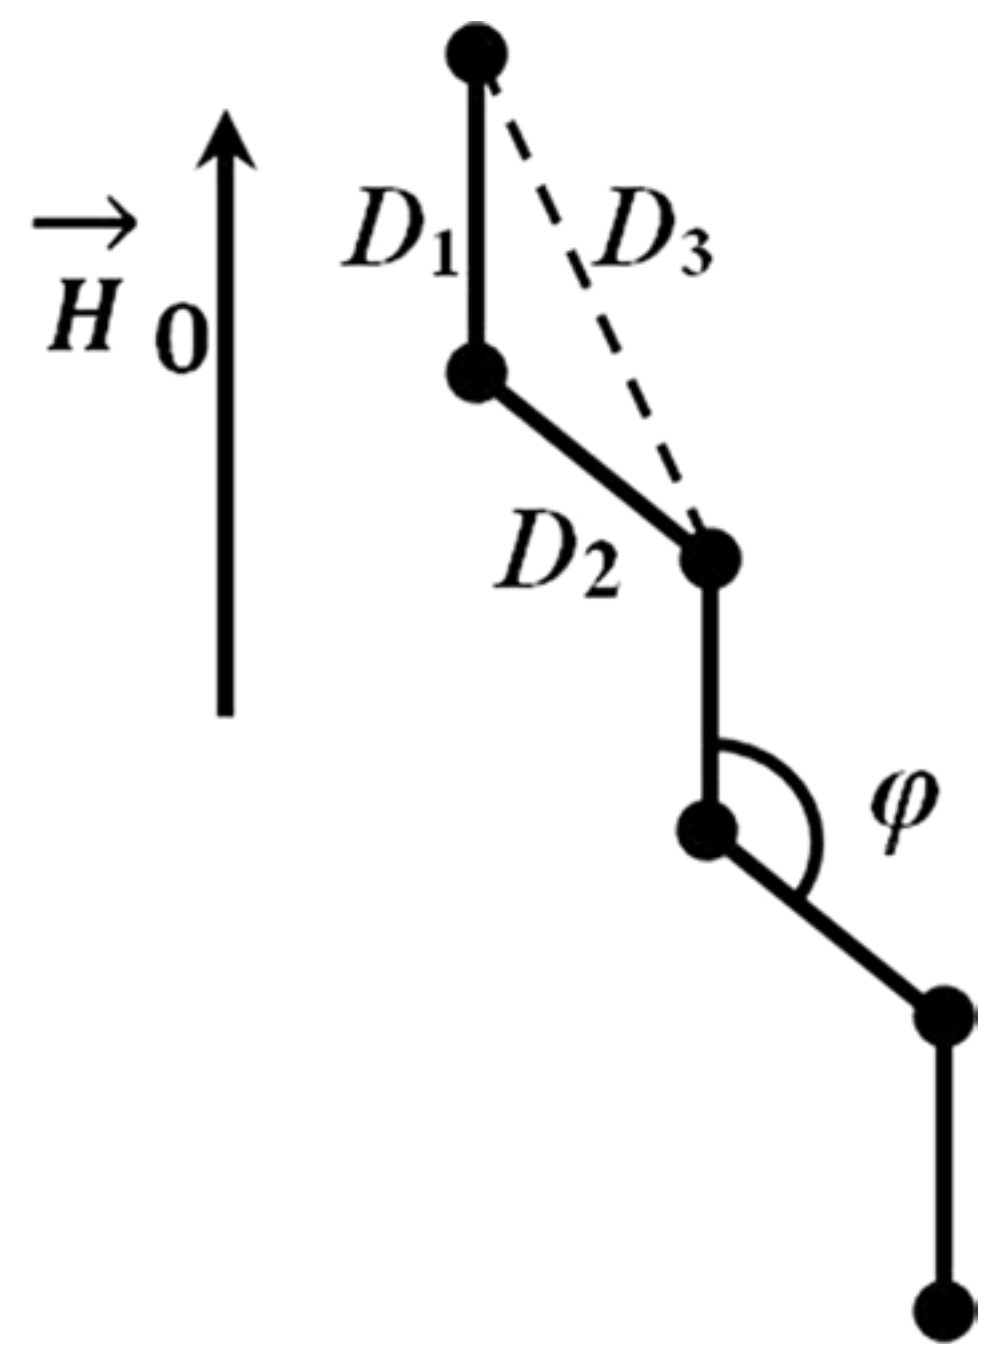
\includegraphics[width=1.0\textwidth]{model-zchain-schema.png}
    \caption{}
    \end{figure}

    \column{0.6\textwidth}
    \begin{block}{Константы взаимодействия}
        $$D_1=\dfrac{\gamma^2\hbar }{r^3}, $$
        $$D_2 = D_1\dfrac{ 3\cos^2 \varphi -1 }{2}, $$
        $$D_3 = D_1 \dfrac{ 3\sin^2 \frac{\varphi}{2} -1}{16 \sin^3, \frac{\varphi}{2}},$$
        где $\gamma$ - гиромагнитное отношение,
        $\varphi$ - угол между соседними связями,
        $r$ - расстояние между соседними спинами в цепочке.
    \end{block}

\end{columns}
\end{frame}
\note{
    Базовый случай это когда одна линия связи направлена вдоль поля. тогда констаты будет самой большой в доль поля.
    Изменяя угол к полю мы можем получить как альтернированную цепочку так и однородную.
    В приближении ближайших и следующих соседей, задача решается аналитически, но она
    не дает полной картины. Поэтому мы решали данную систему численно.
}

\begin{frame}{Альтернированная цепочка (JMR-20)\footnote[frame]{
        G.A. Bochkin and et al., \textit{J. Magn. Res.} \textbf{319}, 106816, (2020)}}
\begin{columns}

    \column{0.4\textwidth}
    \begin{figure}
      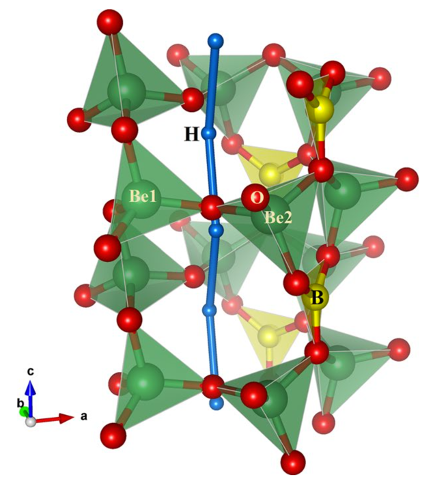
\includegraphics[width=0.85\textwidth]{model-zchain-hambergite-structure.png}
      \caption{}
    %\caption{Hанопора со спин-несущих молекулами во внешнем сильном магнитном поле $\vec B$}
    \end{figure}

    \column{0.6\textwidth}
    \begin{block}{Гамбергит $Be_2BO_3(OH)$ }
        \begin{itemize}
            \item Дипольное взаимодействие между ближайшими спинами протонов в цепи в 17 раз сильнее, чем со спинами окружающих цепей (в худшем случае).
            \item Взаимодействия с остальными окружающими спинами по меньшей мере в 30 раз слабее.
            \item Вклад дипольной связи между спинами в одной и той же цепи доминирует над остальными взаимодействиями.
        \end{itemize}
    \end{block}

\end{columns}
\end{frame}
\note{
    В одномерных цепочках возникают когерентности только $\pm 2$ порядка
    и следовательно дисперсия распределения будет небольшой
    и мы не увидим запутанных кластеров.
    Однако в альтернированная цепочке гамбергита возникают когерентности $\pm 4$ порядка
    и следовательно можно использовать эту модель для исследования многочастичной запутанности.
    The distance to these two protons is 4.49 Å
    The distance between a given chain and surrounding proton chains is at least 2.1 times larger than the distance between neighbors in the chain.

  % JMR 2020
}